\chapter{Background and Related Work}
\label{chap_background}

This chapter provides background and related work regarding three main themes:

\begin{itemize}
\item \textit{The Rise of Hackers and Makers} serves as an introduction to the maker movement which is heavily discussed throughout the thesis. 
\item \textit{Crowdsourcing Problem Solving} provides a classification of systems for crowdsourcing problem solving, a category that includes \textit{This is How}. 
\item \textit{HyperMedia} explores the world of interactive video and HyperMedia, which plays a major role in the design of \textit{This is How}.
\end{itemize}

\section{The Rise of Hackers and Makers}

The ability to innovate is turning into a household commodity. The process of taking an idea and turning it into a product used to be a lengthy process, often measured in years. Today, thanks to availability of a wide range of technologies, and above all the Internet, those processes have changed drastically. 

The first industry to change was the software industry. Contrary to the romantic notion of geeks programming in a garage, building and distributing software before the Internet used to be a lengthy process that required substantial funds. The distribution of software over the Internet has not only decreased the cost of releasing software and software updates but also changed the practice of software development. It has given birth to concept of iterative development in which products are released ``half baked'' and are refined through experimentation and updates. \cite{abrahamsson2002agile}

The Internet has also sped up the development of software by facilitating the accumulation of knowledge and enabling new forms of knowledge sharing and collaboration. Q\&A websites such as StackOverflow\cite{stackoverflow} and code sharing services such as Github\cite{github}, along with the explosion of open source software projects, have allowed programmers to focus on their product rather than tackling issues that have already been solved before. The speeding up of development has also been amplified by the availability of cloud services such as Amazon Web Services\cite{aws}. These allow developers to ``rent'' infrastructure, such as computers and networking equipment, rather than maintaining their own.

While the practice of building and distributing a physical product is inherently different than software, it is being transformed through the availability of tools for digital fabrication. Digital fabrication tools allow for physical objects to be designed digitally on a computer and then fabricated according to design by a dedicated machine. These machines range from numerically controlled milling machines to laser cutters and 3d printers. While various types of these machines have been around since the 1950's, their falling cost, and the introduction of digital control interfaces have increased their availability in recent years and have lowered the threshold for fabricating digital artifacts.

3d printers are perhaps the most associated tools with this transformation. 3d printers, in contrast to other tools like milling machines, use additive manufacturing as opposed to subtractive manufacturing, i.e. they construct an object by adding layers of materials rather than cutting into a block of material. This allows for objects with complex inner structures to be designed and fabricated by people who are not sophisticated designers. 3d printers have gained enormous popularity thanks to their simplicity and the wide availability of cheap models. While they are far from being the ultimate digital fabrication tool, perhaps their greatest contribution is to serve a ``gateway drug'' into the world of digital fabrication. 

With widespread availability of digital fabrication tools, the world of hardware design is starting to mimic the one of software development. Online communities such as Thingiverse\cite{thingverse} and Hackaday\cite{hackaday} allow their members to share designs, learn from others, and collaborate remotely. Prototypes can be built in hours which allows for quick iterative design, similarly to software. 

The proliferation of the above tools and technologies, both in software and hardware, has given birth to a culture of makers and hackers. These individuals, coming from a wide background and carrying diverse skill sets, take pride in the ability to rapidly build prototypes in a non-commercial environment. This culture extends beyond the online communities mentioned above and into real life gatherings and spaces. 

One type of gathering strongly associated with this culture is the Hackathon. Hackathons are events in which hackers gather together for a predefined amount of time, often a weekend, and build prototypes around a predefined subject. These range from commercial Hackathons, organized by companies and aimed at attracting developers to their ecosystem, to social good Hackathons, organized with a specific social goal like improving breast pumps\cite{d2016feminist} or assisting rural communities\cite{hackforwestmass}.   

The maker culture has also triggered the establishment of maker spaces. Maker spaces are physical spaces that serve specific communities by providing the infrastructure for developing software and hardware. These spaces vary in the equipment they possess, some have a single hobbyist 3d printer while others sport hundreds of thousands of dollars worth of equipment such as water-jet and laser cutters. They also vary in their economical model, some are subsidized by the host community or a corporation while other have a paid subscription model. A recent study show that there are around 1,400 maker spaces in the world as of 2016 and that number is growing rapidly\cite{makersbynumbers}.

   \begin{figure}[thpb]
      \centering
      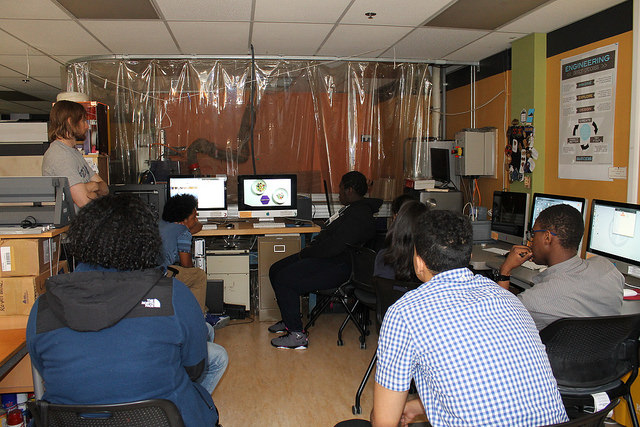
\includegraphics[width=4in]{figures/setc-fablab.jpg}
      \caption{The southend technology center is a small maker space located in the basement of a residential building in Boston, MA \cite{setc}}
      \label{fig_setc_class}
   \end{figure}

   \begin{figure}[thpb]
      \centering
      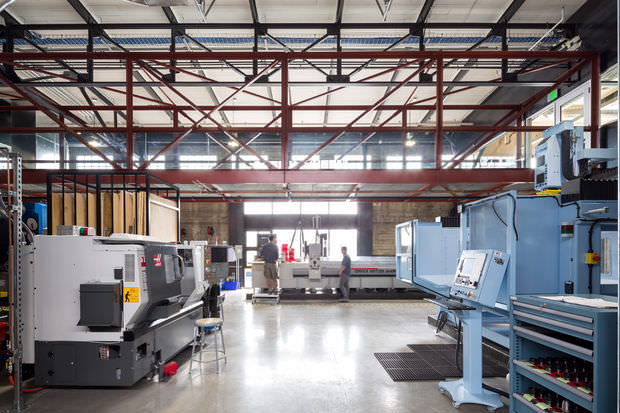
\includegraphics[width=4in]{figures/pier9.jpg}
      \caption{Pier 9 is a 12,000 square-foot maker space used by Autodesk employees and affiliates.\cite{pier9}}
      \label{fig_pier9}
   \end{figure}

\section{Crowdsourcing Problem Solving}

\textit{This is How} is a crowdsourcing system for Brainstorming and Collaboration. It allows makers and nonprofits to exchange knowledge, ideas and skills, and collaborate towards problem solving. In this section I explore existing crowdsourcing systems and their various properties.

In the heart of Crowdsourcing systems are three basic constructs: Initiators, Tasks and Participants. Initiators are organizations or representatives of organizations that publish Tasks which are then performed by Participants. 

In this section focus on Crowdsourcing Systems 

I present various examples of existing systems while characterizing these constructs. What is the motivation of initiators and who are the beneficiaries? How specific are these tasks and what level of skills do they requires? What is the nature of collaboration between participants, if any, and what is their motivation?

In this section I focus on Crowdsourcing Systems that revolve around specific tasks with a clear benefactor, similarly to \textit{This is How}, rather than general systems for collaboration management such as Wikipedia.

\subsection{Simple Tasks Crowdsourcing}

Simple Tasks Crowdsourcing systems are defined as ones where tasks are relatively simple and do not require a significant time commitment. Amazon Mechanical Turk (MTurk) \cite{mturk} is the most well known one. In MTurk, initiators, named Requesters, publish simple tasks to be performed by Participants, called Workers. Tasks carry a monetary reward and don't require any specialized skills or major time commitment. Common tasks include filling surveys and  identifying objects in pictures, these are often used in academic behavioral research.  

Not all of these systems are driven by monetary transactions. Ushahidi is a crowd mapping service driven by social activism\cite{ushahidi}. Ushahidi enables local observers to send geo-tagged reports on incidents during major events. These incidents are plotted on a map accessible via the web and essentially create heat-maps for events. These are monitored by activists and relevant authorities which can act on them. The system has been used in incidents of natural disasters as well in conflict areas during elections. 

These type of systems have also been used in the world of citizen science\cite{sauermann2015crowd}. Galaxy Zoo is one such system that distributes the task of classifying deep space imagery taken by telescopes\cite{galaxyzoo}. Galaxy Zoo utilizes the fact that human observation, with very little guidance, is superior to existing computer vision algorithms in classifying deep space imagery. Since it's inception in 2009, hundreds of millions of photos have been classified. 

\subsection{Bounty Based Crowdsourcing}

In contrast, In bounty based Crowdsourcing systems, tasks tend to be more complex. These systems allow Companies and Organization to publish major challenges they're faced with, along with declared bounty. Multiple participants can offer solutions but only one is chosen by the Client and receives the reward.   

InnoCentive\cite{innocentive}, one such service, is used by companies as big as Dupont and Boeing, who pay up to hundreds of thousands of dollars for creative solutions to the challenges they present. The solvers, as InnoCentive calls them, are often self taught, creative individuals who don't necessarily come from a classic research and design background. This differentiation is what drives their out-of-the-box ideas which these clients seek. \cite{howe2006rise}

Indeed, the great advantage of this approach is democratizing the space of problem solving and lowering the bias of formal training and domain expertise. Marion K Poetz et al (2012)\cite{poetz2012value} show that although crowd sourced ideas tend to be less feasible than traditional expert ones, they show greater novelty and customer benefit. 

\subsection{Distributed Design Crowdsourcing}

The previous mentioned approaches use the Internet to extend their reach, yet they do not tap it's potential of ad-hoc collaboration. Distributed Design Crowdsourcing systems allows for the formation of ad-hoc groups of collaborators working together towards a common goal.  

One of the earliest examples of such a system is ThinkCycle, founded in 2001 \cite{sawhney2002thinkcycle}. ThinkCycle was an initiative started by students at the MIT Media Lab with the aim of bringing the spirit of open source software development into the world of industrial design. It’s key component was an online shared database of problems and evolving design solutions. Similarly to challenge Based systems, each design process started from a challenge posted by a member of the community. However, rather than competing with one another, participants collaboratively came up with ideas and refined them. While ThinkCycle showed some promise it ultimately failed in sustaining a community of problem solvers.

Although ThinkCycle is not active anymore it inspired the birth of similar services. Quirky\cite{quirky} is one that is focused on home automation industry. Members can contribute to ongoing challenges and vote on the significance of contribution of other members. When a product is released all contributors share the profits according to their perceived contribution by the community. 

Openideo\cite{openideo} attempts to utilize the same methodology while tackling global issues.  Their online challenges deal with issues ranging from combating the Zika virus to improving the livelihood of small scale farmers. 

\subsection{Crowdsourcing Systems - Conclusion}

There is a variety of Crowdsourcing Systems that facilitate problem solving. These systems have various characteristics yet they share one, the specificity of the tasks they present. In all the mentioned systems, tasks and challenges are well defined. In this thesis I explore the space of crowdsourcing platforms for clients that don’t necessarily know how to articulate their problems, or indeed, that they face these problems.

\section{HyperMedia}
\begin{quotation}
``There is a joke about the man who has a map of the world ... with a scale of 1 mile to 1 mile. Sometimes video has the same character; it can be difficult to compress in useful ways. Sometimes you have to see all of it to understand any of it.''  \cite{mackay1989eva}
\end{quotation}

This is How makes extensive use of video. Video is inherently linear, it has a well defined length and pace of advancement. This creates various issues I tackle in the Design Considerations chapter. The method I will present is inspired by the world of HyperMedia. In this section I explore its history and related examples.

Since the early days of cinema, filmmakers have attempted to break down the linearity of film. Early attempts took the form of interactive cinema - A non linear cinematic experience that includes decision points in which the viewers choose one of several possible plot directions.

The first interactive cinema movie is considered to be Kinoautomat\cite{cincera1967kinoautomat}, shown in the Montreal World Expo in 1967. At nine points during the film, the screening would stop and a moderator would ask the audience to vote between two possible decisions that represent two possible scenes. The votes were counted and the winning scene would be played next.    

With the introduction of computers and digital media, such experiences became easier to implement. Moreover, they allowed the addition of hyperlinks, images and text layers in addition to the base video layer, marking the move from Interactive cinema to Hypermedia.  

The first Hypermedia experience is often credited to be the Aspen Movie Map\cite{lippman1978aspen} created at the MIT Architecture machine shop in 1978. The Aspen Movie Map was a virtual tour through the streets of Aspen, Colorado, facilitated by a touch display. A user would sit in front of the display and shown a film from the point of view of a car driving through the streets. A touch user interface allowed the user to \"turn\" the direction of the moving car, or focus on a specific building to get more data about it including text and images. 

   \begin{figure}[thpb]
      \centering
      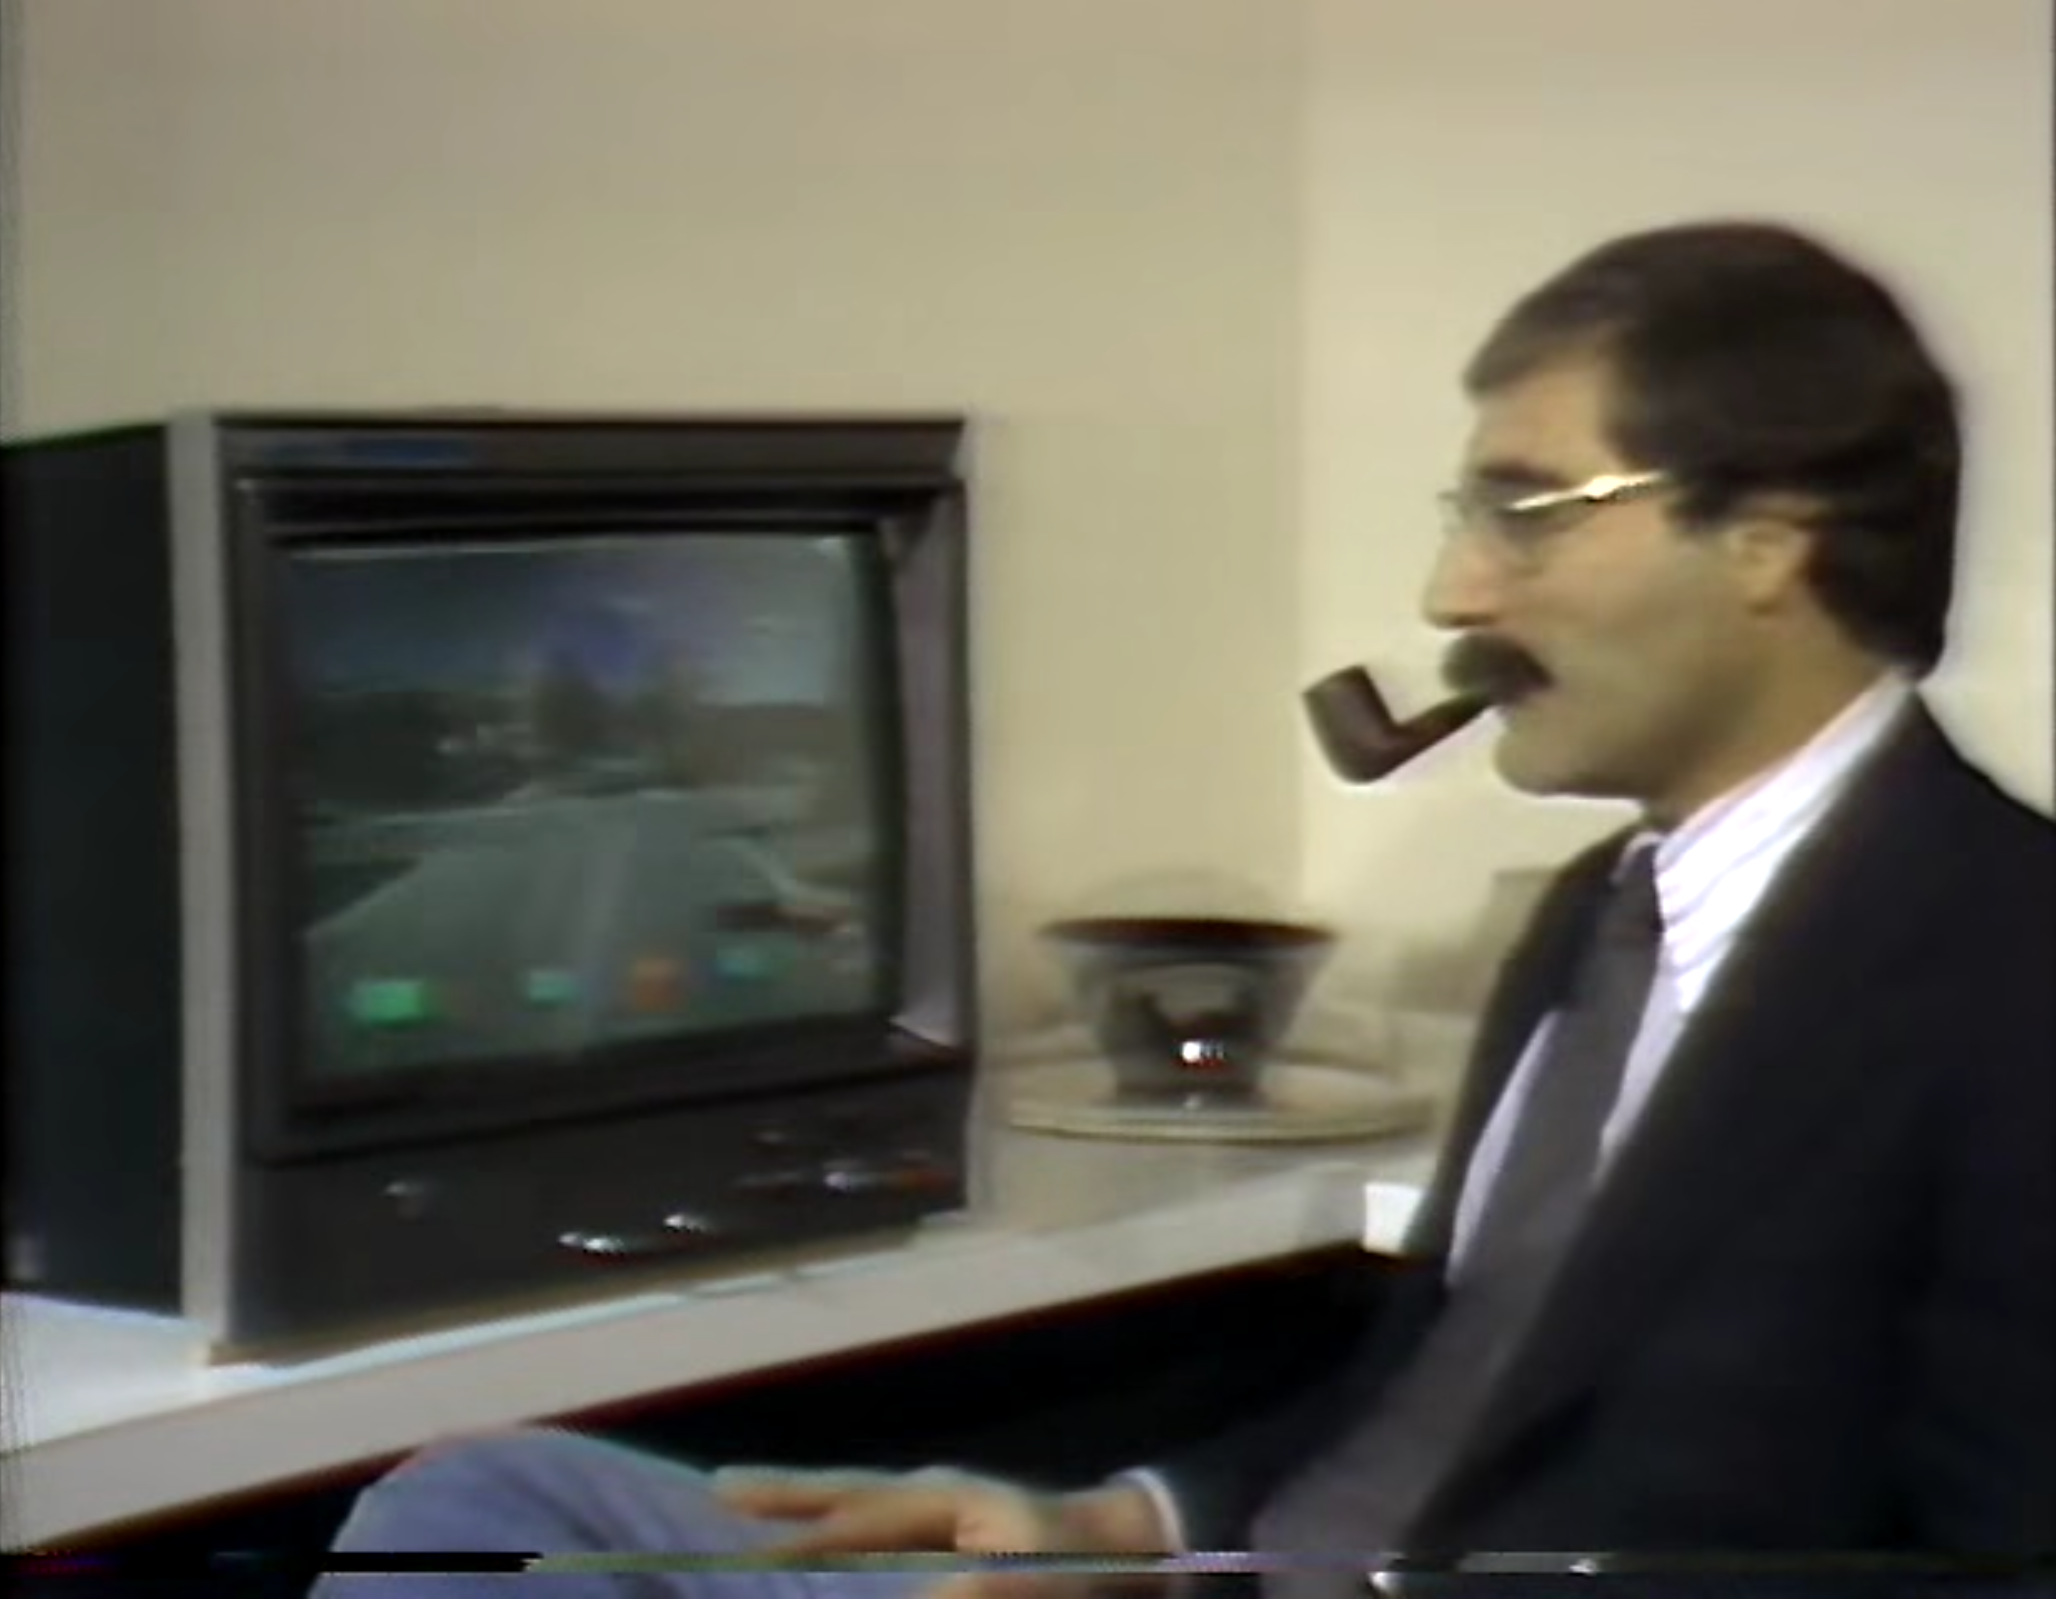
\includegraphics[width=4in]{figures/aspenmoviemap.png}
      \caption{Andy Lippman demonstrating the Aspen Movie Map (1981)\cite{lippman1978aspen}}
      \label{fig_pier9}
   \end{figure}

Hypermedia stayed a focus of the Architecture machine group as they transitioned and became the MIT Media Lab. One notable project led by Glorianna Davenport, was \textit{The Elastic Charles}\cite{brondmo1990creating}, a HyperMedia experience that revolved around a time-lapse journey down the Charles river in Boston. Fifteen students contributed to the project by placing hyperlinks to text, graphics and extra video content on a base film, corresponding to the location portrayed in it. 

With the introduction of the Web, the distribution of HyperMedia using standard technologies became easier. The popular video distribution platform Youtube\cite{youtube} allows video creators to place simple hyperlinks on a specific time and location in their videos that link to other videos published by them. Platforms such as Interlude\cite{interlude} take it a step further by making it easy to create and publish nonlinear videos, where users can make plot decisions and control which scenes are displayed next. Popular streaming service Amazon Video \cite{amazonvideo} have began overlaying TV Shows with hyper links to learn more about the actors relevant to specific scenes being watched.

The above examples show a mixture of two types of interactivity in HyperMedia. In one, such as in Kinoautomat or Interlude, the base video layer can be manipulated by user interactions. In the second, such as in The Elastic Charles, the base layer is static but is overlaid with additional layers of media that provide further information and interactivity. The Aspen movie map combines both. In this thesis I focus on the latter.  



